% !TeX spellcheck = en_US
\section{Data formats for System Biology models}
	\label{sec:background:formats}
	
	At the time this thesis is written, there are two major formats to encode models in \sysbio. With combined over 3237 models in 14439 versions openly available\footnote{\url{http://most.sems.uni-rostock.de/}}, \sbml and \cellml encode a large amount of accessible models in \sysbio.
	Both were independently developed, but serve the similar purpose of supporting basic biochemical network models \citep{Cuellar2003}. Further they use the eXtensible Markup Language \citep{Bray1998} (\xml) as base format, which makes them human readable and enables the use of generic \xml tools and standards \citep{Cuellar2003,Hucka2003} like MathML \citep{Carlisle2003}, XLink \citep{DeRose2010}, and \rdf \citep{Lassila1998}.
	
	Even with serving similar purpose \sbml and \cellml are structured quite different.
	\cellml, for instance, defines a broader scope and features a modular structure, which allows to describe complex interconnected cell models \citep{Cuellar2003}.
	The basic design of \cellml represents a network of interconnected components \citep{Cuellar2003}, which may contain \emph{variables}, and mathematical \emph{equations}. These \emph{equations} determine the behavior of a \emph{component} within a model.
	A \emph{component} is meant to represent a biochemical reaction with it reactants and products, which are represented by \emph{variables}.
	To interlink individual \emph{components} different variables are mapped between them. These mappings are organized in so called \emph{connections}, which are defined between two \emph{components}. Additionally \emph{connections} have to be unique for to given \emph{components}, which means that all mappings between two \emph{components} have to be listed in a single \emph{connections}. (cf. \citet{Cuellar2003})
	
	In contrast to the generic concept of \cellml, \sbml defines more specific design elements.
	The main building blocks are \emph{species}, representing chemical substances, and \emph{reactions}, which are used to describe a transformation of \emph{species} by a mathematical equation. 
	Both are organized in \emph{compartments}, providing a logical or biological container. 
	Another way to control the models behavior is to introduce \emph{rules}. They can be used to establish constraints between \emph{species}, \emph{reactions}, and \emph{parameter}.
	\emph{Parameter} are a tool to further tweak \emph{reactions} and \emph{rules}. They provide a model wide or locally restricted way to externalize quantities, so they can be easily adjusted.
	
	
	
	\begin{comment}
	\begin{itemize}
		\item formats
		\subitem SBML
		\subitem CellML
		\subitem \sedml
		\item everything in XML
		\item semantic annotations
	\end{itemize}
	\end{comment}

\section{Detecting differences in Version Control Systems}
	\label{sec:background:diff}
	
	\subsection{Unix Diff}
	\label{sec:background:diff:unix-diff}
	The essential building block for each Version Control System (VCS) is an algorithm or tool to detect differences between two or more versions, because just storing each version completely is a waste of storage and bandwidth. Further processing change sets enables the system to automatically merge different development branches and therefore making collaboration more efficient.
	
	Nowadays most general-purpose VCS use the \emph{diff} utility, developed as part of UNIX \citep{Chacon2014,OSullivan2009,Collins-Sussman2004}. It is based on the Hunt-McIlroy algorithm, which tries to solve the longest common subsequence problem for two files \citep{Hunt1976}.
	The result is a report of all differences between two files, "expressed as a minimal list of line changes to bring either file into agreement with the other" \citep{Hunt1976}.
	
	\begin{comment}
	\begin{itemize}
		\item Based on solving the longest common subsequence problem
		\item "The program diff reports differences between two files, expressed as a minimal list of line changes to bring either file into agreement with the other" \citep{Hunt1976}
		\item "The central algorithm of diff solves the ‘longest common subsequence problem’ to find the lines that do not change between files" \citep{Hunt1976}
	\end{itemize}
	\end{comment}
	
	\subsection{XML Diff}
	\label{sec:background:diff:xml-diff}
	The problem with the default algorithm used by general-purpose VCS (cf. Section \ref{sec:background:diff:unix-diff}) is, however, that it does only distinguish between text based and binary formats. Hence making none or very little assumptions about the underlying document. Therefore it fails to recognize features, specific to the format. These line-base algorithms tend to be problematic especially for \xml, since line breaks can be neglected, without changing the encoded information. \citep{Ronnau2005}
	
	It can be concluded, that the usual diff algorithm is too fine granular, since it also reacts to changes in the encoding. \xml is represented as hierarchical tree structure and thus it is possible to detect changes based on their position in the tree, rather than a line-number \citep{Wang2003,Chawathe1996,Cobena2002}.
	This can be archived by identifying unchanged subtrees and map them between source and destination version. Going out from those mapped tree, more and more nodes can be matched, under consideration of ancestors, descendants, and labels. Also changed attributes or text-nodes need to be treated differently \citep{Cobena2002}.
	
	\todo{add ref to both examples XyDiff + the other one?}
	
	\begin{comment}
	cf. Cobena2002 \citep{Cobena2002} and \citep{Waltemath2013} in section 2.2.1
	Chawathe et al., 1996 \citep{Chawathe1996}
	\begin{itemize}
		\item "With flat information deltas may be represented simply as sets of tuples or records inserted into, deleted from, and updated in relations. In hierarchical information, we want to identify changes not just to the 'nodes' in the data, but also to their relationships." \citep{Chawathe1996}
		\item "General-purpose version control systems attempt to handle any kind of document and thus make no assumptions about the underlying document format. Usually, those systems distinguish between binary documents and text documents. Appropriate diff algorithms are employed to detect changes between two versions of a document. Those diff algorithms are either line based (for text documents) or byte based (for binary documents). General-purpose version control systems provide good control for line-organized text documents such as source code or latex documents. For XML documents, where the organization into lines can be neglected, 2 line-based version control is inappropriate." \citep{Ronnau2005}
		\item requirements
			\subitem "Within a delta, the exact location of the change must be identified." \citep{Ronnau2005}
			\subitem "XML Structure Information. An XML document is generally a hierarchically structured document, and can be represented in a tree structure. However, an XML document has other features that distinguish it from a general labeled tree. X-Diff introduces the	notion of node signature and a new matching between the trees corresponding to the two versions of a 	document. Together, these two features are used to find the minimum-cost matching and generate a minimum-cost edit script that is capable of transforming the original version of the document to the new version." \citep{Wang2003}
			\subitem "Unordered Trees. Since XML documents can be represented as trees, the change detection problem is related to the problem of change detection on trees." \citep{Wang2003}
		\item "It [the algorithm] tries to detect (large) subtrees that were left unchanged between the old and new versions. These are matched. Starting from there, the algorithm tries to match more nodes by considering ancestors and descendants of matched nodes and taking labels into consideration. Our algorithm also takes advantage of the specificities of XML data. For instance, it knows of attributes and attribute updates and treat them differently from element or text nodes. It also takes into account ID attributes to match elements." \citep{Cobena2002}
	\end{itemize}
	\end{comment}
	
	\subsection{BiVeS}
	\label{sec:background:diff:bives}
	\todo{use the terms source and destination document}
	Continuing on the problem described, in section \ref{sec:background:diff:xml-diff}, the same issue with \xml documents and normal delta algorithms scales to more specific documents and \xml delta algorithms. In this case we look at \xml encoded biological models, either using \cellml or \sbml. Even though algorithms described in the prior section are treating \xml documents as trees, they still lack deeper understanding of a biological model for instance. \bives addresses this issue by building upon XyDiff (cf. section \ref{sec:background:diff:xml-diff}), and by incorporating additional features specific to system biological models, like ontology links, attribute references, and special parts of the model, which are treated atomically \citep{Scharm2015}.
	
	\bives tries to match subtrees of two models, by calculating a hash and a weight for each possible subtree, whereby the weight is always greater than the weight of its children.
	First, the identifying attributes (\xml id attribute and links to bio-ontologies) are used to create a first mapping. Second, this initial mapping is propagated upwards in the document's structure, meaning the connection of a node's children are traversed depth-first and the mapping of these children is suggested for their parents, except if tag-names mismatch. Among the suggested candidates, the most promising mapping is chosen.
	Third the initially generated hashes are used to map remaining subtrees. A priority queue maintains the processing order, so the larger subtrees are mapped first.
	As last step the quality of the mapping is improved by examining the network structure top-down. Each unmapped child is compared to unmatched children in the opposite document and new mappings are created with a maximum distance of $0.9$. This ensures, that completely unrelated nodes are not connected.
	Additionally domain specific mapping rules are in place to apply different strategies for specific characteristics. For instance, certain parts of a model document are treated as atomic units. Whereby different changes in the hierarchical structure are forbidden, which means, that these mappings are unlinked. This is a crucial step, leading to better quality results, when compared to standard \xml delta algorithms.
	
	Finally the different change types are distinguished, by comparing the mappings. An \texttt{insert} is for instance only present in the destination model, but has no mapping to the source model. In contrast a \texttt{delete} can only be found in the source model, certainly not in the destination.
	However these two are called unmapped changes, hence they are identified by the missing link. Opposed to this kind of changes, mapped nodes lead to either an \texttt{update}, \texttt{move}, or no change.
	A \texttt{move} is specified as a case, in which the node is present in both source and destination, but either the parents are not connected, or the order of their siblings is different. An \texttt{update}, however, happens, when the value of an attribute, the content of a text node or the tag name has been alternated.
	
	The resulting \xml delta can be outputted in several formats, including \xml, dot\footnote{\todo{link to graphviz}}, GraphML\footnote{\todo{}}, \json, or as text reports in several markup languages.
	In this work I, will only focus on the \xml output, since it is easy to process and the latest version of \bives also includes \rdf annotations linking to \comodi (cf. section \ref{sec:background:onto:comodi}) \citep{Scharm2015}.
	\todo{include a nice bives figure}
	
	\begin{comment}
	\begin{itemize}
		\item benefits of XyDiff compared to unix-diff
		\subitem problems with XML
		\subitem no deeper "understanding"
		\item cf. \citep{Waltemath2013} (Oxford 2012), \citep{Scharm2015}
		\item algorithm (list of quotes from \citep{Scharm2015})
		\subitem two versions of an XML-encoded model are translated into an internal tree structure. For every node n in the tree, a hash sum n r and a weight n x are calculated 
		\subitem The weight of a node is thus always greater than the weight of its children. As such, the weight represents the size of the corresponding subtree 
		\subitem The hash sum of a node n represents the signature of the subtree rooted at n 
		\subitem While n r unambiguously defines the subtree rooted in n, n r does not need to be unique among all nodes in the tree. Thus, if n r ¼ m r then the subtrees in n and m are identically equal 
		\subitem First, nodes are being mapped with respect to their identifiers 
		\subitem id attributes in the XML documents serve as identifiers. In addition, we also evaluate biological identifiers, specifically links into bio-ontologies 
		\subitem Second, the initial mapping is propagated upwards into the trees. 
		\subitem The connections of a node’s children are evaluated in a depth-first traversal of T 2 . If a node n in T 2 is connected to a node m in T 1 then a mapping of parent ðnÞ to parent ðmÞ is suggested 
		\subitem If, in contrast, n is not connected, we examine the candidates that were previously suggested by the connections of n’s children. 
		\subitem Candidates which have a different tag name than n and candidates which al- ready have a connection are neglected. 
		\subitem Among the remaining candidates, the algorithm chooses the one that received the best suggestions and connects it to n 
		\subitem Third, the algorithm makes use of the initially computed signatures and maps nodes of T 2 on nodes of T 1 
		\subitem A priority queue U is maintained to sort the nodes of T 2 based on their weights. Initially, U only consists of the root node of T 2 . 
		\subitem Unless U is empty, the algorithm repeatedly removes node n 2 U  T 2 with the biggest weight, which represents the biggest subtree in the queue 
		\subitem Fourth, the algorithm improves the quality of the mapping by examining the network structure of T 1 and T 2 in a top-down approach. For every mapping n 2 T 2 on m 2 T 1 , it compares unmatched children of n and m to find missed mappings 
		\subitem The algorithm evaluates the matrix greedily and adds new mappings up to a maximum distance of 0.9. Thus, nodes which have nothing in common will not be connected 
		\subitem Additional mapping rules capture the domain characteristics of the processed data. Following the current specifications for SBML and CellML, we prohibit certain changes in the hierarchical tree of document nodes. Specifically, we treat parts of the model as atomic con- structs for which we define restrictions on possible network operations 
		\subitem This step is a major reason why our algorithm outperforms standard XML diff algorithms. 
		\subitem insert if an entity is present in T 2 but absent in T 
		\subitem delete if an entity is present in T 1 but absent in T 
		\subitem move if a node is present in both documents, but either (i) the parents in the corresponding trees are not connected or (ii) the parents are connected, but the sequence of their siblings has changed 
		\subitem update if the value of an attribute, a text node's content or the tag name of a node was modified
		\subitem After the mapping, we distinguish two types of nodes: mapped nodes and unmapped nodes. Unmapped nodes n 2 T 1 [ T 2 are nodes for which the algorithm could not find a matching node in the opposite tree. These nodes and their attributes correspond to either inserts or deletes, depending on their origin 
		\subitem In contrast, mapped nodes are nodes for which the algorithm did find a matching node in the opposite tree. If the parents of such a mapping of n 2 T 2 onto m 2 T 1 are not connected, or if the se- quence among their siblings has changed, then these nodes are included in the set of moves 
	\end{itemize}
	\end{comment}
	
\section{Managing Versions}
	\subsection{Traditional Version Control Systems}
	\label{sec:background:manage-versions:traditional-vcs}
	
	A Version Control System (VCS), also called Revision Control System, is an automated system to manage multiple versions, or revisions, of information pieces \citep{OSullivan2009}.
	Further, since larger projects are rarely developed by a single person, nearly all VCSs provide mechanisms for collaboration. Version control supports this inherently social endeavor, consisting of continuous introduction, discussion, evaluation of changes, or even undoing them \citep{Collins-Sussman2004}.

	This said, a VCS is a crucial tool for every major project and therefore also of interest in \sysbio \citep{Waltemath2013,Beard2009,Hucka2003,Li2010,Miller2011}.
	All VCS, besides using different files with a version tag, automatically track each version of a file along with relevant meta information. These usually contain the date of change, author and a checksum of the version.
	Originating from this basic feature set, two types of VCS are currently used. On one hand there are centralized VCS, like CVS and its successor Subversion. They focus on one central server, keeping track of all changes. Due to that, working offline is not possible \citep{Collins-Sussman2004}.
	On the other hand a trend around Distributed Version Control Systems (DVCSs) recently evolved. Popular examples for this concept are Mercurial and Git. Their basic architecture does not require a central unit, instead every client keeps a full copy of the version history.
	This structure requires strong merge algorithms, since a merging multiple change sets in always required when the base version of different clients differs \citep{OSullivan2009}.
	But DVCSs do not completely abandon the idea of a central server, instead it is treated as a place to share changes with other teammates, still allowing for experiments or off-mainstream development.
	
	\begin{comment}
	\begin{itemize}
		\item benefits of version control systems
			\subitem \todo{elaborate}
			\subitem "The need for model version control has been previously discussed in research groups facing model evolution in computational biology (Beard et al., 2009; Cuellar et al., 2006; Hucka et al., 2010; Li et al., 2010; Miller et al., 2011). In general, VCSs such as Subversion (http://subversion.apache.org/) (SVN)" \citep{Waltemath2013}
		\item simple file storage
			\subitem storing files next to each other in the file system
			\subitem "-version1", "-version2", "-final"
			\subitem no meta information stored along with versions (author, time stamp)
			\subitem collaboration causes problems
			\subitem but: simple and quick
		\item SVN
			\subitem client/server architecture
			\subitem collaboration possible, through branching and merging capability
			\subitem reverse-delta storage
			\subitem no offline work possible
		\item GIT
			\subitem distributed VCS
			\subitem reverse-delta storage with version graph
			\subitem build for heavy collaboration by using information from the version graph for merging
			\subitem \todo{refer to version-graph later, when explaining db concept}
			\subitem \url{https://git-scm.com/book/en/v2/Git-Internals-Plumbing-and-Porcelain}
	\end{itemize}
	\end{comment}
		
	\subsection{Challenges traditional VCSs face with Systems Biology models}
	\label{sec:background:manage-versions:challenges}
	
	Even with VCSs being heavily used in most software development projects nowadays, \sysbio struggles to adapt those systems for a variety of reasons.
	The most obvious one would be the missing awareness among Systems Biologists, due to their strong foundation in Biology. Means the priority for them might be less in good data management, but more on understanding biological processes.
	Besides social aspects, there are also a lot of technical reasons, why common VCSs fail to perform well in \sysbio.
	
	All currently used VCSs rely by default on the \emph{UNIX diff} tool (cf. Section \ref{sec:background:diff:unix-diff}) to identify changes between versions. Since all in this work used data formats for \sysbio models are using \xml to encode them (cf. Section \ref{sec:background:formats}), the commonly used \emph{UNIX diff} is widely unsuitable (cf. Section \ref{sec:background:diff:xml-diff}).
	But even specialized algorithms for delta generation of \xml files, may fail to perform well (cf. Section \ref{sec:background:diff:xml-diff}). To improve this situation the algorithms need to take domain specific knowledge into account and be specifically fitted to the representation format \citep{Waltemath2013}.
	If the used algorithm is not fitted to the format, changes in the encoding may be detected and flood the change log. Often these encoding changes do not affect the model and will therefore render the change log useless.
	But even with sufficient knowledge about the domain and suitable \xml delta algorithms, it may be impossible to determine the importance or the scope or impact of a change. Hence a VCS, tailored for \sysbio, is not only supposed to store different revisions of a model, but also to "reflect the temporal evolution [...] and present model changes to the user" \citep{Waltemath2013} in a clear way, a semantic taxonomy is required, to communicate these changes (cf. to \comodi, Section \ref{sec:background:onto:comodi}).
	
	Currently there are 2 major approaches to store version information \citep{Waltemath2013}:
	The very first approach suggests to store a change log of minor changes in the model itself \citep{Beard2009}.
	The second suggests to keep track of changes within a repository, which is currently more applied. However, neither of these methods meet all requirements, mentioned above.
	
	\begin{comment}
	\begin{itemize}
		\item SVN and GIT are using unix-diff -> not suitable for XML files (cf. XML diff section)
		\item no semantic information about the changes (cf. comodi)
		\item no domain specific knowledge to improve mapping of different XML-tree branches
			\subitem important for good detection of tree branch movement etc. 
			\subitem "A model VCS should be tailored to existing model representation formats, which are typically XML and RDF based. It should furthermore reflect the temporal evolution of a model and present model changes to the users." \citep{Waltemath2013}
			\subitem "These
			common changes are detected by the LCS algorithm, but they are in fact irrelevant for the model’s history and would be neglected by entity-based algorithms. In other words, although being successfully used for source code version control, LCS is not suitable for XML version control (Chawathe et al., 1996)." \citep{Waltemath2013}
		\item As proposed in \citep{Waltemath2013} there are 2 major approaches to keep track of changes:
			\subitem keeping track of (minor) changes in the model itself
			\subitem tracking versions in the repository
	\end{itemize}
	\end{comment}

\section{Ontologies in Computer Science}
	The idea of a semantic web was first introduced by Tim Berners-Lee et al. in 2001 \citep{Berners-Lee2001}, he described the idea of a federated knowledge graph, which can, opposed to the traditional web, be parsed and "understood" by computer algorithms. The aspired goal was to establish a network of agents, which are able to retrieve information from anywhere, analyze them and provide the user with an 
	aggregated information or even an decision, ready for approval.
	Merging mentioned federated data sources is by far not easy. Even though the semantic web introduces a number of standards and formats, it is fairly difficult to link information from different data sources. Because there might be differences in the used schema, the type of data does not entirely overlap, or they describe information on a different level of abstraction \citep{Berners-Lee2001}.
	To overcome this issue, ontologies were introduced. "In philosophy, an ontology is a theory about the nature of existence, of what types of things exist; ontology as a discipline studies such theories" \citep{Berners-Lee2001}.
	In contrast computer science and more specifically the semantic web research, has borrowed this term, but uses it to describe a hierarchically structured group of terms or a taxonomy, together with a set of reasoning rules.
	
	To communicate and use these taxonomies and rule sets the \owl standard was introduced \citep{Bechhofer2004,Bechhofer2009}. It encodes all terms, their relations, attributes and verbal descriptions, as well as all rules.
	
	\sysbio uses this technology to annotate already machine readable data files, instead of data sources available over the web. They hereby serve the purpose of giving additional information about parts of a model or the model itself. The variety of available ontologies ranges from biological species identification with \emph{Systems Biology Ontology} (SBO\footnote{\url{http://purl.bioontology.org/ontology/SBO}}), the description of simulation algorithms and proceeding with \emph{Kinetic Simulation Algorithm Ontology} (KiSAO\footnote{\url{http://purl.bioontology.org/ontology/KISAO}}), to the characterization of dynamics with the \emph{Terminology for the Description of Dynamics} (TEDDY\footnote{\url{http://purl.bioontology.org/ontology/TEDDY}}) \citep{Courtot2011}.
	
	\begin{comment}
	
	\begin{itemize}
	\item definition
		\subitem formal definition, properties and relation of entities
	\item use of BioOntologies cf. Courtot \citep{Courtot2011}
	\end{itemize}

	\todo{citep owl standard, when explaining comodi import}
	\todo{http://msb.embopress.org/content/7/1/543.short for ontology overview}
	\end{comment}
	
	\subsection{\comodi}
	\label{sec:background:onto:comodi}
	
	\begin{figure}[h]
		\centering
		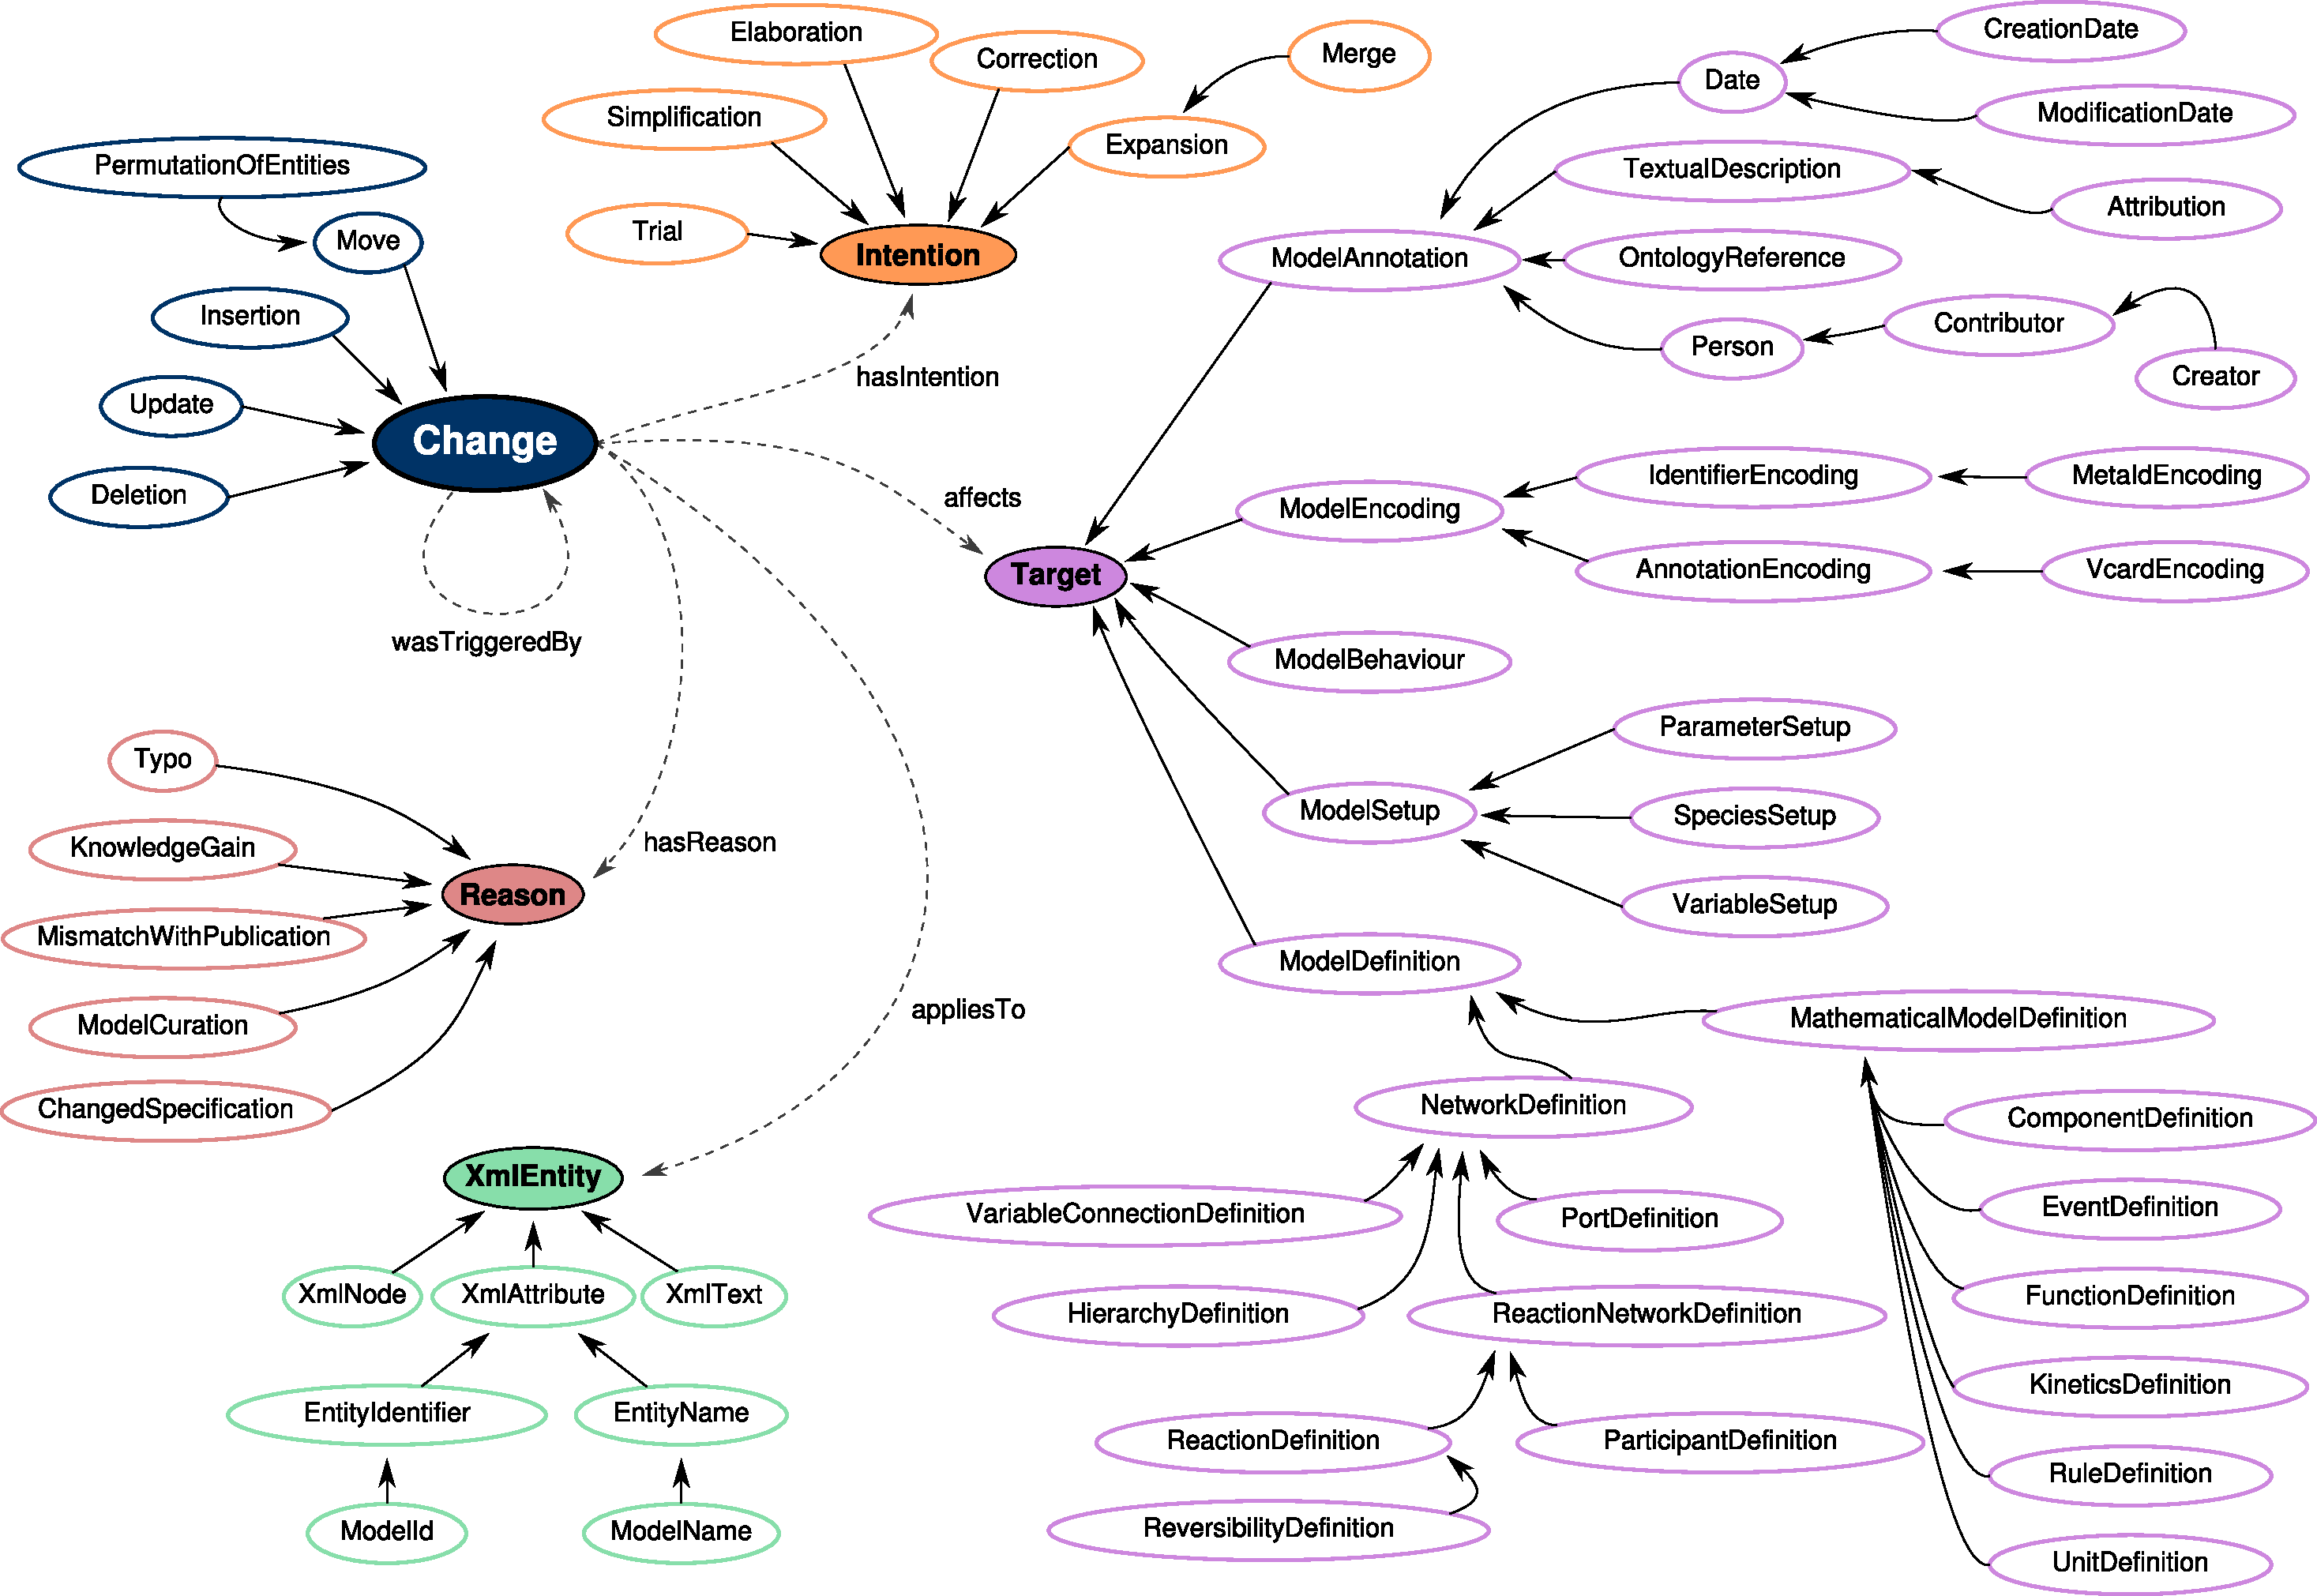
\includegraphics[width=\textwidth,keepaspectratio]{resources/comodi-overview.pdf}
		\caption[Visualisation of \comodi]{Visualization of all classes of the \comodi ontology, taken from \citealt{Scharm2016}. \url{http://purl.uni-rostock.de/comodi/2016-03-12}}
		\label{fig:background:onto:comodi}
	\end{figure}
	
	Identifying the position and the existence of changes is only the first step in deeper understanding, the evolution of a document or biological model. To truly explain this evolution, the historical development, reason, purpose, and target of a modification are important. 
	However, to formalize these information a standardize vocabulary is required. Preferably in a structure, that can be used for automatic processing of the data, making them "more accessible, sharable and interoperable" \citep{Scharm2016}.
	An ontology is well suited tool for building interlinked and structured vocabularies, which useful in semantic annotations and therefore enrich otherwise plain data with meaning.
	
	\comodi was developed to provide exactly this layer of semantic information to differences between two versions of a biological model, allowing to store the essential meaning of a change together with its potential implications.
	\citeauthor{Scharm2016} are reasoning, how important it is to track these additional information to changes. A modification of parameters or the underlying reaction network may change the outcome, breaking the reproducibility of this model. To prevent this it is important to detect certain changes and 
	react correspondingly.
	Further, \citeauthor{Scharm2016} argue, that change records may help to predict, if modifications have an impact on the simulation result, which can then be communicated accordingly -- improving the trust of scientist in the reuseability of this model.
	However, with an increasing size of the change records, the difficulty to perceive the relevance of certain changes increases. Therefore it is important to add more information to these changes, allowing for ranking and filtering them.
	
	In order to fulfill all these requirements, \comodi is organized in four branches, linking from the main concept \texttt{Change}: \texttt{XmlEntity}, \texttt{Intention}, \texttt{Reason}, and \texttt{Target}. A visualization of all classes an their hierarchy is shown in Figure \ref{fig:background:onto:comodi}.
	The concepts of \texttt{Intention} and \texttt{Reason} both express the purpose of a change. While \texttt{Intention} focuses on possible effects in the future, the \texttt{Reason} indicates the cause -- therefore expressing past events leading to the annotated change. For instance a \texttt{Reason} for a change might be a \texttt{MismatchWithPublication} causing a parameter update.
	In contrast \texttt{Target} and \texttt{XmlEntity} both describe the entity, a change is pointing to.
	More specific the \texttt{Target} branch is able to distinguish between 5 layers, which can modified in terms of a change: the first layer expresses changes of the formal \texttt{ModelEncoding}, this could be used to express an update of the used \sbml version.
	On the second layer, \texttt{ModelAnnotation} is meant to express changes on the semantic layer, e.g. annotations. 
	On the contrary further layers refer to changes affecting the actual model behavior. Beginning with \texttt{ModelDefinition}, which refers to changes in the biological system, for instance the reaction network. Whereby \texttt{ModelSetup} describes modifications in the simulation setup, e.g. initial values and parameters. The last branch, \texttt{ModelBehaviour}, links to the TEDDY ontology \citep{Courtot2011} and therefore makes it possible to captures changes in the dynamics of the system.
	Additionally to the different branches, \comodi allows to model causality of changes by introducing a \texttt{wasTriggeredBy} relation, which expresses "mutual dependencies". However, \comodi does not provide any terms to describe provenance information, but it can be easily incorporated with ontologies build for this purpose.
	
	
	
	\begin{comment}
	\begin{itemize}
		\item cf. \citep{Scharm2016}
		\item  They clarify the intended semantics of the data, which makes the data more accessible, sharable, and interoperable 
		\item An ontology is a tool to provide meaning to data, the information of which can then be subjected to algorithmic processing
		\item We believe that a similar approach should be taken for the semantic description of differences between versions of a model. Using the semantic layer to describe changes in a model allows for storing meaning together with possible implications of these changes.
		\item It is important to track these changes for a number of reasons. Changes in parametrisations or on the underlying network may lead to a situation where the original results are not reproducible anymore.
		\item With respect to simulation results, change records can help to predict modifications in the simulation outcome. Finally, a good communication of model changes increases the trust of scientists wishing to reuse a model for their own purposes.
		\item  as the list of changes increases it becomes harder to grasp their relevance. To address this problem, we present an ontology to annotate the changes identified with the BiVeS algorithm.
		\item  it is always possible to specify the XML entity that is subject to a change. 
		\item COMODI is organised into four branches around the central concept Change: XmlEntity, Intention, Reason, Target
		\item Intention and Reason both indicate the purpose of a change. On the one hand, the Intention specifies the aim of a change, particularly with respect to consequences in the future. In our example, the intention of modifying the parameter value is a Correction. On the other hand, a Reason specifically focuses on the cause of a change. In our example, a MismatchWithPublication caused an update of the parameter value.
		\item COMODI basically distinguishes between five layers in a model document, that can be subject to a change:
		\item Finally, different changes might be linked to each other if they have mutual dependencies.
		\item The COMODI ontology is specifically designed for the annotation of differences between versions of a computational model in the life sciences.
		\item Some information can directly be inferred and thus be annotated automatically with BiVeS
		\item  The ontology terms specify the type of change for each detected difference. Usually, a combination of COMODI terms from different branches is necessary to characterise a change sufficiently.
		\item COMODI terms can also be applied to differences detected between models in any other encoding format, including even code from proprietary languages such as MATLAB 
		\item COMODI cannot, however, be used to encode provenance, such as information about the user who changed the model or information about the tool used to update the file. It can, however, easily be coupled with ontologies for provenance.
	\end{itemize}
	\end{comment}